% Papers should not exceed 8000 words (approx. 16 pages).

\PassOptionsToPackage{unicode=true}{hyperref} % options for packages loaded elsewhere
\PassOptionsToPackage{hyphens}{url}
%
\documentclass[12pt]{scrartcl}
\usepackage{lmodern}
\usepackage{amssymb,amsmath}
\usepackage{ifxetex,ifluatex}
\usepackage{fixltx2e} % provides \textsubscript
\ifnum 0\ifxetex 1\fi\ifluatex 1\fi=0 % if pdftex
  \usepackage[T1]{fontenc}
  \usepackage[utf8]{inputenc}
  \usepackage{textcomp} % provides euro and other symbols
\else % if luatex or xelatex
  \usepackage{unicode-math}
  \defaultfontfeatures{Ligatures=TeX,Scale=MatchLowercase}
\fi
% use upquote if available, for straight quotes in verbatim environments
\IfFileExists{upquote.sty}{\usepackage{upquote}}{}
% use microtype if available
\IfFileExists{microtype.sty}{%
\usepackage[]{microtype}
\UseMicrotypeSet[protrusion]{basicmath} % disable protrusion for tt fonts
}{}
\IfFileExists{parskip.sty}{%
\usepackage{parskip}
}{% else
\setlength{\parindent}{0pt}
\setlength{\parskip}{6pt plus 2pt minus 1pt}
}
\usepackage{hyperref}
\hypersetup{
            pdftitle={How logical and pragmatic inferences determine acceptability judgements},
            pdfauthor={Mojmír Dočekal},
            pdfborder={0 0 0},
            breaklinks=true}
\urlstyle{same}  % don't use monospace font for urls
\usepackage{longtable,booktabs}
% Fix footnotes in tables (requires footnote package)
\IfFileExists{footnote.sty}{\usepackage{footnote}\makesavenoteenv{longtable}}{}
\usepackage{graphicx,grffile}
\makeatletter
\def\maxwidth{\ifdim\Gin@nat@width>\linewidth\linewidth\else\Gin@nat@width\fi}
\def\maxheight{\ifdim\Gin@nat@height>\textheight\textheight\else\Gin@nat@height\fi}
\makeatother
% Scale images if necessary, so that they will not overflow the page
% margins by default, and it is still possible to overwrite the defaults
% using explicit options in \includegraphics[width, height, ...]{}
\setkeys{Gin}{width=\maxwidth,height=\maxheight,keepaspectratio}
\setlength{\emergencystretch}{3em}  % prevent overfull lines
\providecommand{\tightlist}{%
  \setlength{\itemsep}{0pt}\setlength{\parskip}{0pt}}
\setcounter{secnumdepth}{0}
% Redefines (sub)paragraphs to behave more like sections
\ifx\paragraph\undefined\else
\let\oldparagraph\paragraph
\renewcommand{\paragraph}[1]{\oldparagraph{#1}\mbox{}}
\fi
\ifx\subparagraph\undefined\else
\let\oldsubparagraph\subparagraph
\renewcommand{\subparagraph}[1]{\oldsubparagraph{#1}\mbox{}}
\fi

% set default figure placement to htbp
\makeatletter
\def\fps@figure{htbp}
\makeatother

\usepackage{linguex}
\usepackage{stmaryrd}
\usepackage{qtree}
\usepackage{natbib}

%\usepackage{covington}
\newcommand{\cond}[1]{\textsc{#1}}
%\let\oldShaded\Shaded
%\let\endoldShaded\endShaded
%\renewenvironment{Shaded}{\tiny\oldShaded}{\endoldShaded}
\let\oldverbatim\verbatim
\let\endoldverbatim\endverbatim
\renewenvironment{verbatim}{\tiny\oldverbatim}{\endoldverbatim}

\title{How logical and pragmatic inferences determine acceptability judgements\thanks{ACKNOWLEDGMENTS, GRANT -- to be added after review.}}
\providecommand{\subtitle}[1]{}
\author{Mojmír Dočekal}


\begin{document}
\maketitle

\hypertarget{intro}{%
\section{Intro}\label{intro}}

In this article I focus on a problem of dividing negative dependent expressions into two classes: (i) \textit{n-words} like Czech \textit{nikdo } `nobody' or Romanian \textit{nimeni} `nobody' (glossed as n-person) in \Next[a] from \cite{fualuaus2016fragment}; (ii) Negative Polarity Items (NPIs) like Czech \textit{sebemenší šance} `slightest chance ' or Romanian \textit{vreun} `any' in \Next[b] (Ibid.). Despite the long research traditions on both types of expressions (for NPIs see \citealt{heim1984note}, \citealt{ladusaw1992expressing}, \citealt{kadmon1993any}, \citealt{krifka1995semantics}, \citealt{giannakidou1997landscape}, \citealt{lahiri1998focus}, \citealt{gajewski2011licensing}, \citealt{chierchia2013logic}, \cite{crnivc2014against} among many others; for n-words see \citealt{laka1990negation}, \citealt{zeijlstra2004sentential}, \citealt{zeijlstra2008negative} among others) there is still not an consensus on the relationship between the two items. 

\ex. \ag. \textbf{Nimeni} nu a venit.\\
n-person not has come\\
`Nobody came.' \bg. * \textbf{Vreun} student nu a venit.\\
NPI student not has come\\
`*Any student didn't come.' \hfill [Ro]

Nevertheless, it seems to be settled that the division between n-words and NPIs correlates with the division between syntactic licensing and semantic licensing along the following lines:

\begin{enumerate}
\def\labelenumi{\arabic{enumi})}
\item
  \textbf{n-words} are syntactically negative dependent expressions;
\item \textbf{N(egative) P(olarity) I(tems)} are semantically negative dependent expressions;
\end{enumerate}

Some languages lexicalise the difference between NPIs and n-words, as was shown in the example \Last but sometimes the distinction manifests itself only via stress (and consequently) focus marking. An example of the second strategy is in \Next from \cite{giannakidou2017landscape} where the non-focused expression \textit{kanenan} `anybody' is (according to standard criteria) NPI while the focused expression \textit{KANENAN} `n-person' behaves as a n-word.

\ex. \ag. Dhen idhe \textbf{kanenan} o Janis.\\
not saw NPI-person the John\\
`John didn't see anybody' \bg. Dhen idhe \textbf{KANENAN} o Janis.\\
not saw n-person the John\\
`John didn't see anybody \emph{at all}.' \hfill [Gr]

Next to the classification of n-words as being basically licensed in syntax (either via agreement or some other standard syntactic process) and NPIs as semantically dependent expressions (occurring only in environments with specific monotonicity properties) there is as well an agreed \textbf{criterion} of teasing apart the two classes, one of a recent formalizations can be found in \cite{giannakidou2017landscape} -- see \Next, their example (16). The criterion is partially meaning based and partially relies on context felicity of n-words. Its working will be exemplified in the following sections.

\ex. X qualifies as an n-word iff:\label{nwords-npi-crit} \a. X can be used with structures
with sentential negation or other X with meaning equivalent to one
\(\neg\) \b. X provides a negative fragment answer.

In this article I discuss mainly experimental evidence from Czech which allows us to answer a research question: do languages like Czech (where the evidence to differentiate between n-words and NPIs is very limited) distinguish between n-words and NPIs (particularly the class of NPIs called strong NPIs)?

The article is organized as follows: in the first, more theoretically based part (Section \textbf{\nameref{npis-vs.n-words-theory}}) I will illustrate the empirical criteria distinguishing n-words and NPIs, then I will tease apart so called weak NPIs from strong NPIs and lastly will introduce the basic observations about Czech and negative dependent expression. The Sections \textbf{\nameref{neg-raising}}, \textbf{\nameref{fragment-answers}} and \textbf{\nameref{likelihood-scenarios}} will be more of the experimental linguistic character, they are heavily based on the joint work with Jakub Dotlačil (partially reported in \citealt{dovcekal2016experimental}, \citealt{docekaldotlacilsubedin}, \citealt{docekaldotlacilsubber}). In concreto, I will report the experimental evidence for distinguishing n-words from NPIs stemming from three classes of phenomena: (i) Neg-Raising contexts; (ii) Fragment answers; (iii) Likelihood manipulated contexts. The nature of this article is more overview-like, the details about statistics, design of the experiments, etc. can be found in \cite{dovcekal2016experimental}, \cite{docekaldotlacilsubedin}, \cite{docekaldotlacilsubber} and \cite{docekalsafratovaoli}.

\hypertarget{npis-vs.n-words-theory}{%
\section{NPIs vs.~n-words: theory}\label{npis-vs.n-words-theory}}

\hypertarget{n-words}{%
	\subsection{n-words:}\label{n-words}}

Let's start with introducing some important pieces of linguistic knowledge concerning n-words, the expressions which are generally taken as syntactically dependent on negation and which are different both from negative quantifiers on one hand and from NPIs on the other hand.

N-words crucially differ from Germanic negative quantifiers as the following contrast in \Next shows: English verbal negation and a negative quantifier in \Next[a] yield only double negation reading while the word for word translation of \Next[a] into Czech with n-word \textit{nikoho} `anybody' and verbal negation in \Next[b] is interpretable only with one negation scoping wide over the whole sentence as is clear from the predicate logic formalization. Generally, n-words are syntactically dependent expressions which occur only in languages where some form of negative concord is attested.

\ex. \a. John didn't see nobody. \hfill [En]\\
 \(\neg \exists x[Person'(x) \wedge \neg See'(John,x)]\)
 \b. John nikoho neviděl. \hfill [Cz]\\
 \(\neg \exists x[Person'(x) \wedge See'(John,x)]\)

The distinction between n-words and NPIs already mentioned in the criterion in \ref{nwords-npi-crit} is illustrated in \Next: \Next[b] illustrates the un-availability of NPIs as fragment answers versus the perfect acceptability of n-words in the same context in \Next[d] -- Czech translation of \Next[a] -- \Next[b] mini-dialogue.

  NPIs \(\neq\) n-words:

\ex. \a. Whom did you talk to? \b. *Anybody.
\c. S kým jsi mluvil? \d. S nikým.

There are at least two influential theories of n-words: the first one treats n-words as non-negative indefinites (predicate at type \(\langle e,t\rangle\)) which are required to be in the scope of clause-mate negation (so called roofing requirement from \cite{ladusaw1992expressing}, see \cite{giannakidou1997landscape} for an historical overview). The second type of theory compares n-words to agreement markers which nicely explains their locality requirements, basically their need to be licensed syntactically by clause-mate negation. The second type of approach is developed in  \cite{zeijlstra2004sentential} and \cite{zeijlstra2008negative}. In this article I will follow the syntactic agreement approach even if nothing hinges too much on the particular framework as far as it constrains the distribution of n-words to clauses with overt verbal negation. This locality constraint is one of the usually mentioned contrast between n-words and NPIs since unlike  NPIs which just need to be in a scope of negative element, n-word need a local negation as the following contrast from \cite{giannakidou2017landscape} shows.


\ex. \ag. Dhen prodhosa mistika {[}pu eksethesan
{[}kanenan/*KANENAN{]}{]}\\
Not betrayed.1sg secrets that exposed.3pl anybody/n-body\\
`I didn't revela secrets that exposed anybody.'

It should be noted that the locality requirement of n-words varies across languages but n-words in Slavic languages the  locality is very strict  as observed already by \cite{progovac1993negative}. So unlike in Spanish, Italian or Greek where the licensing of n-word sometimes (especially in case of subjunctive embedding) can span from a negation on root verb to n-words in embedded clauses, such licensing is ungrammatical in Slavic languages, see the following examples from Czech.

\ex. \ag. *Petr neřekl, že nikdo přišel.\\
Petr neg.said that n-body came\\
`Petr didn't say that anybody came.' \bg. *Petr nechce, aby tu nikdo
byl.\\
Petr neg.wants C.subj here n-body were\\
`Petr doesn't want anybody were here.'


\hypertarget{npis}{%
\subsection{NPIs}\label{npis}}

A prototypical example of a Negative Polarity Item (NPI) is English expression \emph{any} -- see the seminal work of \cite{kadmon1993any} (and there for older references). If an NPI occurs in a sentence without negation it results in an ungrammatical sentence -- \Next. If it occurs in a negated sentence like in \NNext, the only interpretation is a scope of \textit{any} under negation: \NNext[a] vs. the sentence's un-acceptable interpretation in \NNext[b].

\ex. *Peter visited anyone.

\ex. Petr didn't visit anyone. \a.
\(\neg \exists x[Person'(x) \wedge Visit'(Peter,x)]\)
\b. \#$\exists x[Person'(x) \wedge \neg Visit'(Peter,x)]$

Next, negation is not the only expression licensing NPIs (which at least in the case of so called weak NPIs) sets NPIs apart from n-words which are licensed only by negation. Compare the following Czech paradigm in \Next where the NPI/minimizer \textit{sebemenší šance} `slightest chance' contrasts with the n-word \textit{žádnou} `n-adj'. The NPI licensing expression in \Next[a] is the quantifier \textit{málo studentů} `few students'. The negation and other  NPI licensing expressions share the property of reversing the direction of entailment in their argument. Notice how negation reverses entailment in the Table 1. Because of this NPIs licensors entailment reversion property their essential property is called downward entailing (DE) and is generally accepted by scholars as the most probable common denominator of NPIs environments (since \citealt{ladusaw1992expressing}).


\ex. \ag. Málo studentů mělo sebemenší šanci složit tu zkoušku. \\
few students had slightest chance to.pass the exam\\
`Few students had slightest chance to pass the exam.'
\bg. \# Málo studentů mělo žádnou šanci složit tu zkoušku. \\
few students had n-adj chance to.pass the exam\\
`Few students had slightest chance to pass the exam.'

\begin{figure}


\begin{longtable}[]{@{}cccc@{}}
\toprule
\begin{minipage}[b]{0.03\columnwidth}\centering
p\strut
\end{minipage} & \begin{minipage}[b]{0.03\columnwidth}\centering
q\strut
\end{minipage} & \begin{minipage}[b]{0.37\columnwidth}\centering
(p \(\wedge\) q) \(\rightarrow\) (p \(\vee\) q)\strut
\end{minipage} & \begin{minipage}[b]{0.46\columnwidth}\centering
\(\neg\)(p \(\vee\) q) \(\rightarrow\) \(\neg\)(p \(\wedge\) q)\strut
\end{minipage}\tabularnewline
\midrule
\endhead
\begin{minipage}[t]{0.03\columnwidth}\centering
1\strut
\end{minipage} & \begin{minipage}[t]{0.03\columnwidth}\centering
1\strut
\end{minipage} & \begin{minipage}[t]{0.37\columnwidth}\centering
1\strut
\end{minipage} & \begin{minipage}[t]{0.46\columnwidth}\centering
1\strut
\end{minipage}\tabularnewline
\begin{minipage}[t]{0.03\columnwidth}\centering
0\strut
\end{minipage} & \begin{minipage}[t]{0.03\columnwidth}\centering
1\strut
\end{minipage} & \begin{minipage}[t]{0.37\columnwidth}\centering
1\strut
\end{minipage} & \begin{minipage}[t]{0.46\columnwidth}\centering
1\strut
\end{minipage}\tabularnewline
\begin{minipage}[t]{0.03\columnwidth}\centering
1\strut
\end{minipage} & \begin{minipage}[t]{0.03\columnwidth}\centering
0\strut
\end{minipage} & \begin{minipage}[t]{0.37\columnwidth}\centering
1\strut
\end{minipage} & \begin{minipage}[t]{0.46\columnwidth}\centering
1\strut
\end{minipage}\tabularnewline
\begin{minipage}[t]{0.03\columnwidth}\centering
0\strut
\end{minipage} & \begin{minipage}[t]{0.03\columnwidth}\centering
0\strut
\end{minipage} & \begin{minipage}[t]{0.37\columnwidth}\centering
1\strut
\end{minipage} & \begin{minipage}[t]{0.46\columnwidth}\centering
1\strut
\end{minipage}\tabularnewline
\bottomrule
\end{longtable}

	\centering Table 1
\end{figure}


In natural language the reasoning of monotonicity is frequently applied in relation to set, subsets and supersets. Notice the predicate logic implications in \Next which corresponds to the patterns from the propositional calculus. If there is some \textit{x} in the intersection of \textit{P} and \textit{Q} denotation then necessarily there is an \textit{x} in \textit{P} and \textit{Q} union \Next[a]. And if there is no \textit{x} in \textit{P} and \textit{Q} union, then there cannot be any \textit{x} in their intersection \Next[b]. So in a positive sentence (in predicate logic non-negated formula) the entailment goes from an subset (intersection) to a superset (union) while in a negated sentence, the entailment is reversed and proceeds from a superset (union) to its subset (intersection). A natural language example is in \NNext: denotation of NP \textit{red wine} is a subset of a NP \textit{wine} denotation and in a positive sentence \NNext[a] the entailment is from a subset to a superset, not vice versa: \NNext[b]. In a negated sentence the entailment reverses: \Next[c] entails \Next[d].

\ex. \a. $\exists x[P(x) \wedge Q(x)] \rightarrow \exists[P(x) \vee Q(x)]$
\b. $\neg \exists[P(x) \vee Q(x)] \rightarrow \neg \exists x[P(x) \wedge Q(x)]$

\ex. red wine \(\rightarrow\) wine \a. John likes red wine.
\(\rightarrow\) John likes wine. \b. John doesn't like red wine.
\(\not\rightarrow\) John doesn't like wine. \c. John doesn't like wine.
\(\rightarrow\) John doesn't like red wine.

The general condition stating that NPIs occur in  Downward Entailing (DE) environments can be stated like \Next.

\ex. Fauconnier-Ladusaw's Licensing Condition: An NPI is only
grammatical if it is in the scope of an \(\alpha\) such that
\(\llbracket \alpha \rrbracket\) is DE.

The downward monotonic and upward monotonic reasoning in case of quantifiers works like this:  upward monotonic quantifier allow reasoning from  subsets to supersets while downward monotonic quantifier from  supersets to subsets: \Next. Natural language examples of upward, downward and non-monotonic quantification are presented in \NNext.

\ex. \a. det A: upward entailing iff for any B, C (\(B \subseteq C\))
\(Det\ A\ B \Rightarrow Det\ A\ C\) \b. det A: downward entailing iff
for any B, C (\(B \subseteq C\)) \(Det\ A\ C \Rightarrow Det\ A\ B\) \c.
if not upward or downward monotonic \(\rightarrow\) non-monotonic


\ex. Upward/Downward entailing and Non-monotonic determiners: \a. some:
Some toys are blue \(\Rightarrow\) Some toys are colored \b. few: Few
toys are colored \(\Rightarrow\) Few toys are blue \c. exactly \emph{n}:
Exactly three toys are blue \(\not\leftrightarrow\) Exactly three toys
are colored

It is important to notice that  monotonicity properties belong to a position in a sentence and they are computed compositionally: so a position in a sentence can be upward monotonic even if it occurs in a scope of downward entailing quantifier. In \Next the object position is in a scope of two DE quantifiers and consequently is upward monotonic, as the validity of the entailment pattern shows.

\ex. \a. {[}\(\downarrow\) At most three detectives arrested
\(\downarrow\){[}fewer than four \(\uparrow\){[}criminals{]}{]}{]} \b.
\(\rightarrow\){[}\(\downarrow\) At most three detectives arrested
\(\downarrow\){[}fewer than four \(\uparrow\){[}humans{]}{]}{]}

\hypertarget{weak-npis}{%
\subsection{Weak and Strong NPIs}\label{weak-npis}}

There is a class of NPIs, so called weak NPIs with prototypical English examples like  \emph{any, ever, \ldots{}}. Weak NPIs occur in all Downward Entailing environments as illustrated in \Next.

\ex. \a. Bill didn't \textbf{ever} say \textbf{anything}. \b. No student
\textbf{ever} said \textbf{anything}. \c. Few students \textbf{ever}
said \textbf{anything}. \d. At most 5 students \textbf{ever} said
\textbf{anything}. \e.*Between 5 and 10 students \textbf{ever} said
\textbf{anything}. \f. *Some/*all/*most students \textbf{ever} said
\textbf{anything}.

The second class of NPIs instantiated by English expressions like  \emph{in weeks}, additive \emph{either}, and punctual \emph{until} are so called strong NPIs and as the name suggests, they occur only in a subset of environments where weak NPIs are grammatical as illustrated in \Next.


\ex. \a. Bill didn't leave \textbf{until his birthday}. \b. No student
left \textbf{until his birthday}. \c. ??Few students left \textbf{until
their birthdays}. \d.*At most 5 students left \textbf{until their
birthdays}. \e.*Between 5 and 10 students left \textbf{until their
birthdays}. \f.*Some/*most/*all students left \textbf{until their
birthdays}.

The logical property which licensors of strong NPIs share (negation and \textit{no} in \Last) is a strengthened form of entailment reversal and usually is named anti-additivity. In using anti-additivity as the necessary condition for strong NPI acceptability I follow seminal work of \cite{zwarts1998three}. There's a popular alternative explanation of strong NPIs and their behavior in \cite{gajewski2011licensing} which describes their stricter distribution via downward entailing properties but checked both in at-issue meaning and in the presupposition/implicature part of the meaning. I'll stick to the classic theory of anti-additivity here: the definition is in \Next. \NNext illustrates the anti-aditivity (the quantifier \textit{no} is anti-additive since negation is always anti-additive as is clear from deMorgan's law: $\neg(p \vee q) \leftrightarrow (\neg p \wedge \neg q)$). But DE quantifiers like \textit{few} in \ref{ex:few} are not anti-additive -- imagine a scenario with 10 students, three of them dancing and three of them smoking, then $\vee$ part of \ref{ex:few} is false while $\wedge$ part of \ref{ex:few} is true.



\ex. Anti-additive function:
\(F(x \vee y) \leftrightarrow F(x) \wedge F(y)\)

\ex. No student smokes or drinks \(\leftrightarrow\) No student smokes
and no student drinks.

\ex. Few students smoke or drink \(\not\leftrightarrow\) Few students
smoke and few students drink \label{ex:few}

a

\hypertarget{npis-vs.n-words-modularity}{%
\subsection{NPIs vs.~n-words}\label{npis-vs.n-words-modularity}}

Returning now to the broader question of distinguishing between NPIs (negative dependent expressions licensed in semantics via notions like monotonicity plus anti-additivity) and n-words (negative dependent expressions licensed in syntax via agreement), it is acknowledged that such a distinction corresponds nicely with a well established modularity architecture of a grammar where usually we  distinguish between different forms of ill-formedness such as syntactic, semantic, \ldots{} which is located in different modules of grammar. But the picture is not so clear when we consider recent theories of NPI licensing where the  logical properties correlate with syntactic acceptability of NPIs. In concreto: if ungrammaticality of NPIs in upward entailing environments is due to lack of the right monotonicity properties in them, then we are in fact linking the domains of semantics with syntax. And in some theories (Heim/Crnič) of NPIs licensing where the licensing of NPIs is postulated via presupposition the linking goes even further: between the licensing in pragmatics with syntactic acceptability. Recent theories of NPIs (CHIERCHIA) and strong NPIs (Gajewski) seem to point in the same direction.

Before we'll move to the experimental part of the article, let's have an outlook of Czech data scrutinized in much more detail in the series of experiments I will report. In Czech there are two candidates both at first sight reasonable for the NPI or n-word status: \textit{ani jeden} `not even one' and žádný `no'. As the following example demonstrates, both require clause-mate negation, so both can be either n-words or strong NPIs (the embedded clauses of communicative verbs can be shown to be non-anti-additive: details to follow).

\ex. \ag. Petr neviděl ani jednoho/žádného studenta.\\
Petr neg.saw even one/any student\\
`Petr didn't see any student.' \b. *Ani jeden/*žádný student přišel.\\
Not even one/any student came. \c. Petr neslyšel, že *ani jeden/*žádný
student přišel.\\
Petr didn't hear that even one/any student came.

So it is well conceivable that four logical possibilities of classifying \textit{ani jeden} `not even one' and \textit{žádný} `no' are reasonable. Czech tradition like \cite{havranek1960slovnik} can be interpreted as the following table suggest, so basically treating both types of expressions as syntactically dependent on negation.


\begin{longtable}[]{@{}lll@{}}
\toprule
item/status & NPIs & n-words\tabularnewline
\midrule
\endhead
\emph{ani jeden} & X & \(\checkmark\)\tabularnewline
\emph{žádný} & X & \(\checkmark\)\tabularnewline
\bottomrule
\end{longtable}

And as it is clear from the previous discussion the division between n-words and strong NPIs is subtle -- the only other clause-mate environment (next to negation) which passes the test of anti-additivity are prepositions like English \textit{without} (compare the equivalence of: \textit{John left the pub without paying and saying good bye $\leftrightarrow$ John left the pub without paying or John left the pub without saying good bye}). So it is reasonable to ask a research question like \Next. Neg-concord languages like Czech (and generally all Slavic languages) do employ negative dependency on negation via n-words, so is there a reason for a language to maintain a set of expressions which do nearly the same job but are licensed in semantics? In the rest of the article I will argue for the positive answer to the question: the experimental evidence clearly shows that \textit{ani jeden} `not even one' expression pattern like strong NPIs, not like n-words.

\ex. Research question: do strict neg-concord languages even allow grammaticalization of Strong NPIs?

\hypertarget{experimental-evidence}{%
\section{Experimental evidence}\label{experimental-evidence}}

In the three following sections I will discuss the experimental evidence which allows us to tease apart n-words from NPIs. First in the section \ref{neg-raising} I will report an evidence coming from the behavior of NPIs in the Neg-raising constructions: Neg-raising (NR) is a primarily interpretational phenomen where a negation of verbs like \textit{think, believe} or \textit{want} is most saliently understood as scoping over their embedded verb (\textit{I don't want to leave} $\approx$ \textit{I want not to leave}, compared with a lack of such interpretation in case of non-NR predicates: \textit{I don't say I will leave} $\not\approx$ \textit{I am saying that I will not leave}). In the following section \ref{fragment-answers} the evidence for distinguishing between n-words and NPIs will come from their different acceptability as fragmentary answers to questions. And in the last section \ref{likelihood-scenarios}, the two classes will be shown to behave differently with respect to their entailment and likelihood properties.

\hypertarget{neg-raising}{%
\subsection{Neg-raising}\label{neg-raising}}

Because NPIs are licensed in semantic part of the grammar engine, they are (ceteris paribus) expected to be able to be licensed at long distance. N-words as syntactically dependent on negation have to obey strict locality conditions unlike NPIs. And even more importantly, if the licensing of NPIs happens in semantics, their licensing should be sensitive to properties of their embedding verbs, in case of NR-predicates, NPIs should appear in the embedded clauses of NR-predicates but are predicted to be un-acceptable in the embedded clauses of non-NR predicates (verbs of communication or causation). If we construe such long distance licensing, the expected pattern should look like the one in the table below: n-words cannot be licensed across clausal boundary, while NPIs can but in case of NR-predicates, we expect sharp difference between predicates like \textit{want, believe, \ldots} and non-NR predicates like \textit{hear, say, force, \ldots}.

\begin{longtable}[]{@{}lll@{}}
\toprule
environment/status & NPIs & n-words\tabularnewline
\midrule
\endhead
NR embedded & \(\checkmark\) & X\tabularnewline
non NR embedded & X & X\tabularnewline
\bottomrule
\end{longtable}

The experimental results which bear on this issue are in a bigger details summarized in \cite{dovcekal2016experimental}. Let's call this experiment, Experiment 1. Experiment 1 consisted of 5 conditions demonstrated in \Next, one of the items of the experiment. The experiment tested acceptability of sentences containing NPIs.

\ex. \ag. \textbf{Ztratila} se \textbf{ani} jedna ovce.\\
Lost SE not-even one sheep\\
`A single sheep is missing.' \bg. \textbf{Neztratila} se \textbf{ani}
jedna ovce.\\
neg-lost SE not-even one sheep\\
`Not a single sheep is missing.' \c. Nový bača v Tatrách
\textbf{nechce}, aby se ztratila \textbf{ani} jedna ovce.\\
new shepherd in Tatras neg-wants C SE lost not-even one sheep. \d. Nový
bača v Tatrách si \textbf{nemyslí}, že se ztratila \textbf{ani} jedna
ovce.\\
new shepherd in Tatras SI neg-think C SE lost not-even one sheep \e.
Nový bača v Tatrách \textbf{neříká}, že se ztratila \textbf{ani} jedna
ovce.\\
new shepherd in Tatras neg-say C SE lost not-even one sheep

The sentences represent 5 environments listed below:

\begin{enumerate}
\def\labelenumi{(\Alph{enumi})}
\tightlist
\item
  a positive sentence (A)
\item
  a negative sentence (B)
\item
  a clause embedded under negated NR predicates of intention and
  judgement/obligation (e.g.~\emph{want, advise}) (C)
\item
  a clause embedded under negated NR predicates of opinion
  (\emph{believe}) (D)
\item
  non-NR predicates (E)
\end{enumerate}

Experiment 1 tested only NPIs: \emph{ani jeden} was one two NPIs in it, the second one \textit{až do} `until' + time expression is not important for this article. The descriptive statistics of Experiment 1 is visualized in Figure 1: x-axis represents the 5 conditions and y-axis represents the 5-point Likert scale (1 \ldots the least acceptable, 5 \ldots the most acceptable). The boxplots summarize the acceptability in the usual manner. As is evident from the graph, Condition A was the least acceptable, Condition B best accepted, all other conditions somewhere in the interval between the two extremes. The most important difference is the one between the conditions C and D and E where E represents non-NR predicates and was perceived as less acceptable by native speakers. This seems to be result of un-licensed NPI in the embedded clauses of non-NR predicates.

\begin{figure}
\centering
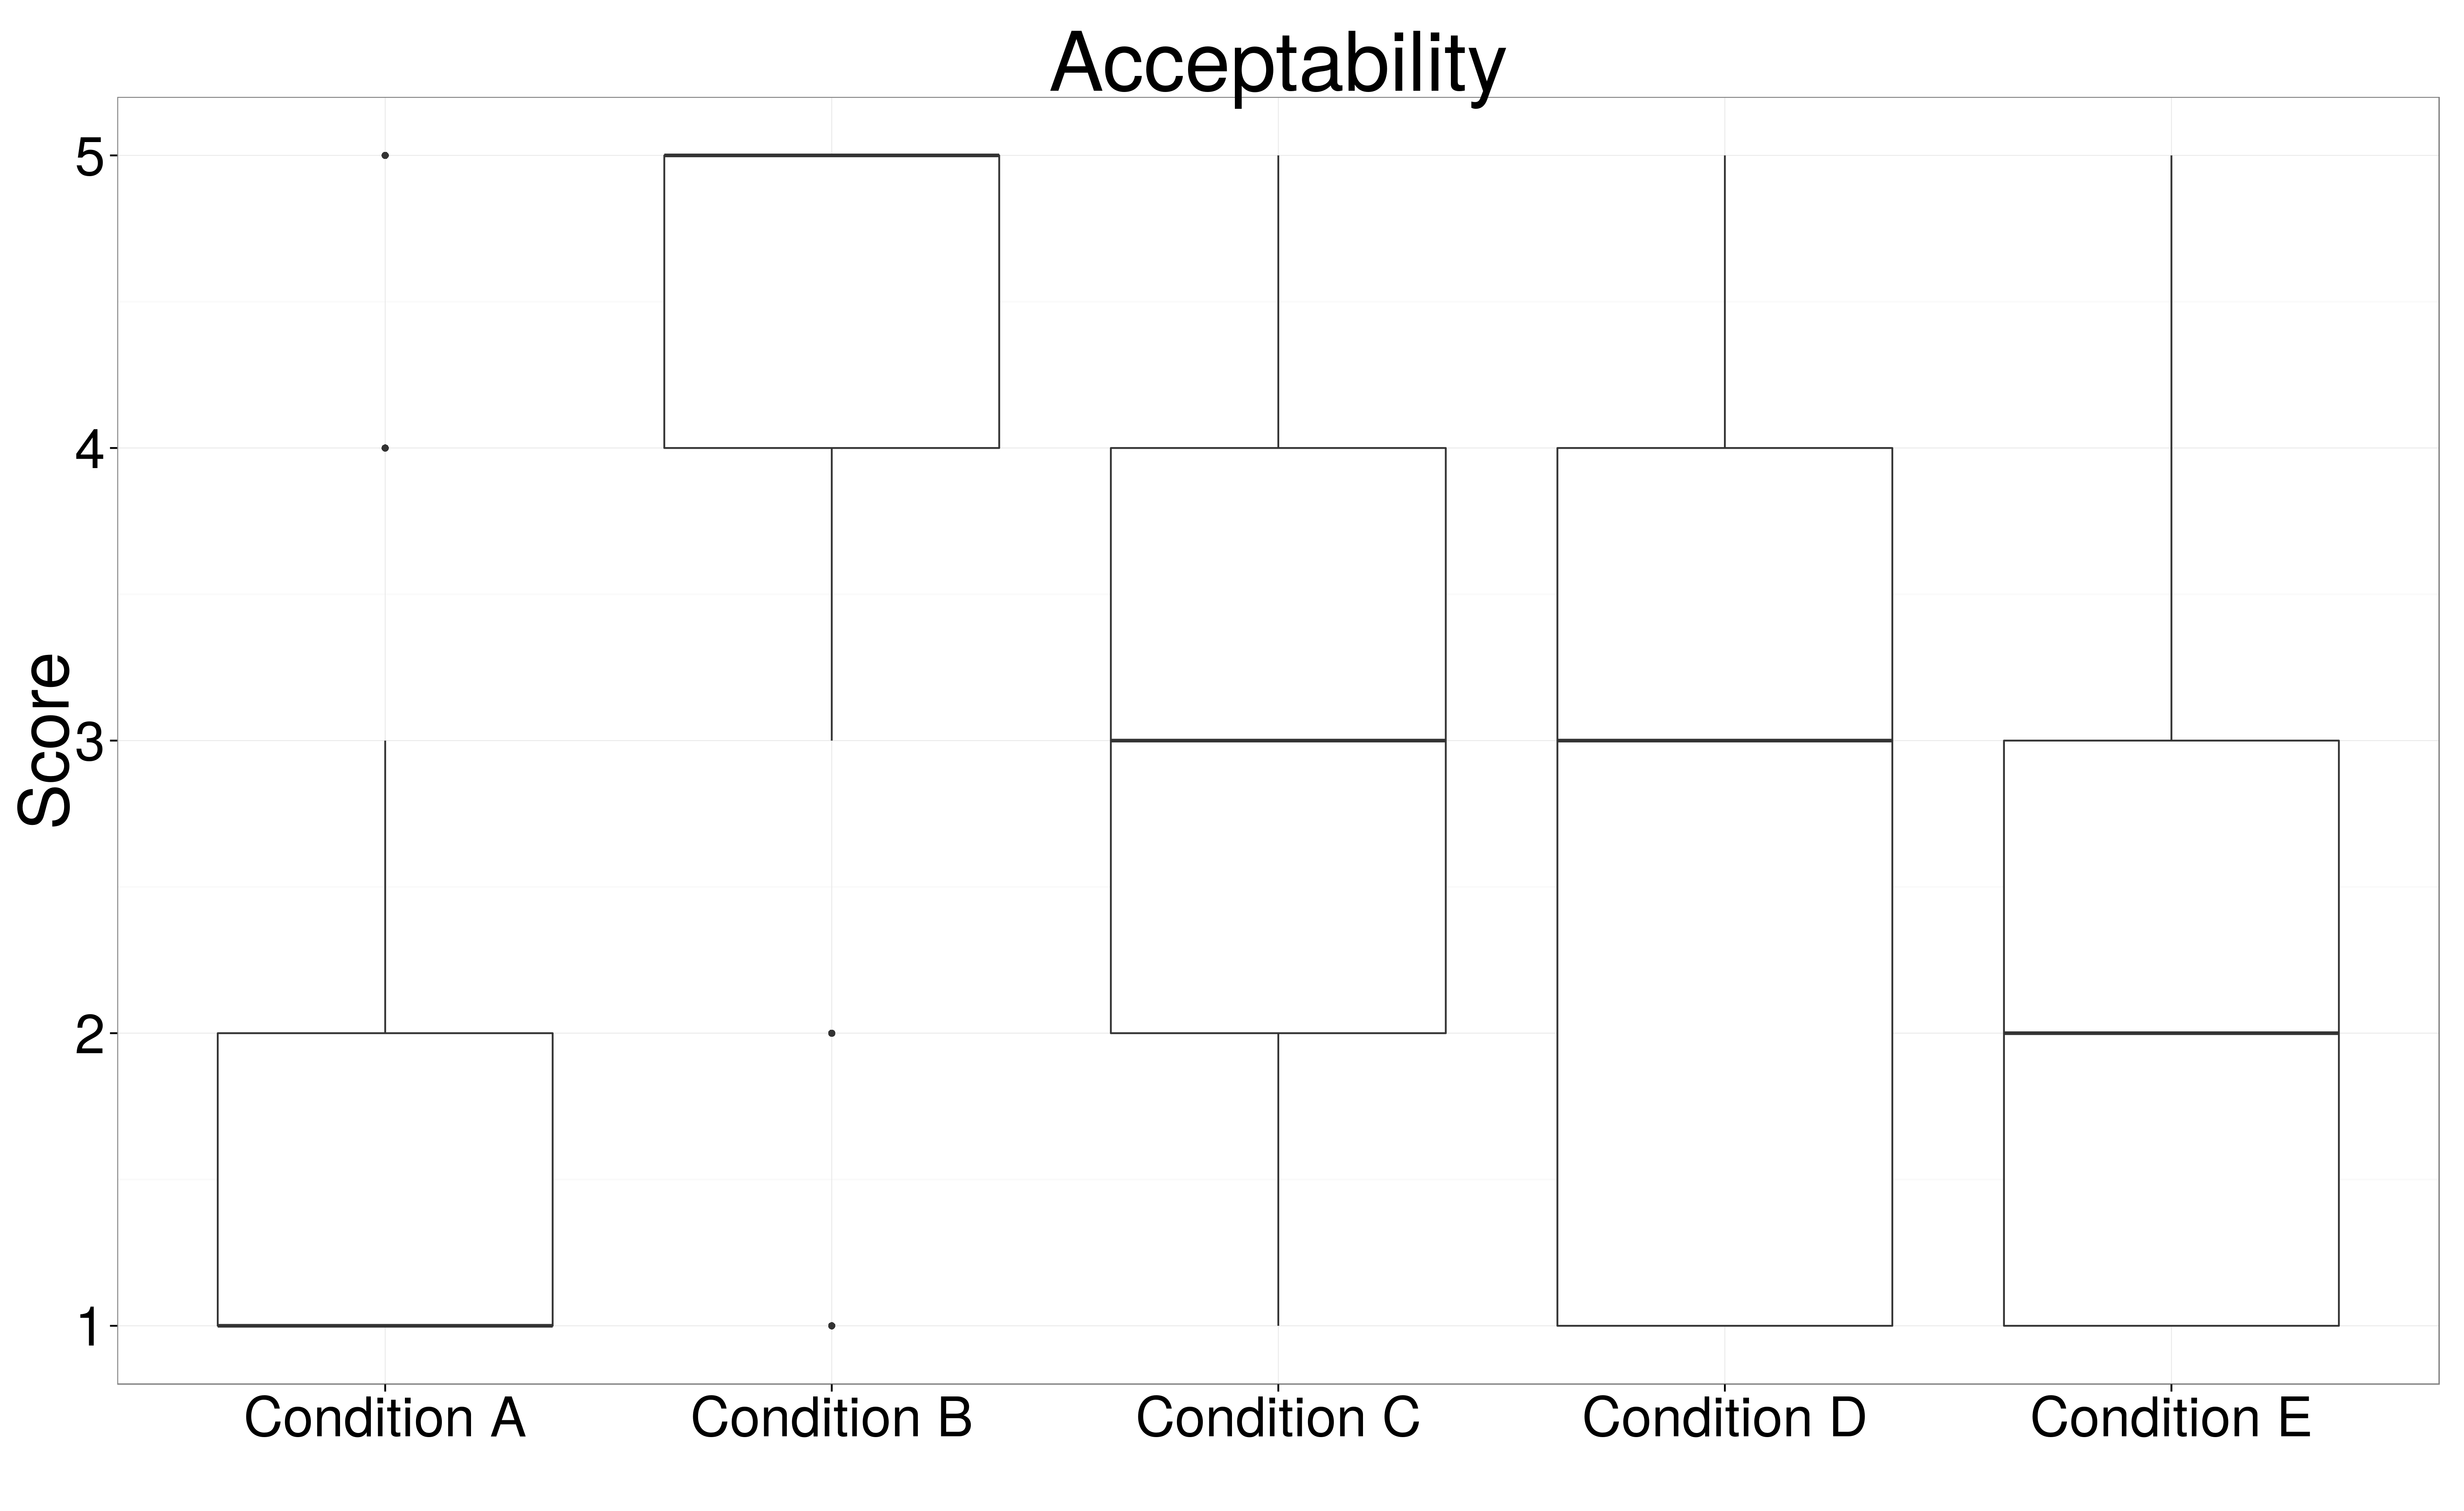
\includegraphics{include/boxplot-exp1.png}
\caption{Experiment 1}
\end{figure}

The results of the experiment can be theoretically explained in the the scalar approach to NR (\citealt{horn1973semantic}, \citealt{romoli2012soft}, \citealt{romoli2013scalar}). In the scalar theory of Neg-raising  NR predicates (beside the assertion -- \Next[a]) contribute the  excluded middle (EM) implicature to the semantic composition (\Next[b]). And finally the   alternatives generated by the implicature are exhaustified by EXH -- \NNext.

\ex. \a. \(\llbracket P \rrbracket = \lambda p\lambda x.\square_x[p]\)
\b.
\(Alt(NR)=\{\lambda p\lambda x.\square_x[p],\lambda p\lambda x.[\square_x[p] \vee \square_x[\neg p]]\}\)

\ex.
\(EXH(Alt(p))(p)(w) = p(w) \wedge \forall q \in Excl(p,Alt(p))[\neg q(w)]\)

I will illustrate the mechanics of scalar theory of NR on an example item from the Experiment 1: \Next. Formula in \NNext[a] shows the alternatives generated by the excluded middle implicature from \LLast[b]: it is the negated at-issue meaning ($\neg want_s[p]$) and the excluded middle part ($\neg(want_s[p] \vee want_s[\neg p])$). The excluded middle in this case formalizes the involvement of the subject \textit{s}: he either wants thee proposition \textit{p}, or he wants the negation of \textit{p} but he cannot un-interested with respect to \textit{p}. The excluded middle for other classes of NR-predicates has analogous meaning: opinionatedness for \textit{know}/\textit{believe}, clear intentions for \textit{plan}, etc. Compare lack of such excluded middle meaning in predicates of communication: a speaker can say \textit{p} or neg \textit{p} but he can be silent about \textit{p} as well. \Next[b]) then shows the exhaustification of the alternatives: the at-issue meaning remains the same but the excluded alternative is negated -- the usual strenghtening of the sentence meaning via negating its alternatives. The at-issue meaning and double negated excluded middle alternative then (via deductive reasoning) yield the semantic low scope of negation in the embedded proposition. So, as a consequence of exhaustification of NR predicate and its excluded middle implicature, the negation is of the NR predicate interpreted as having low scope (semantically).
  

\ex. `A new shepherd in Tatra mountains doesn't want even one sheep to
be missing.' \(\neg want_s[p]\) .

\ex. \a.
\(Alt(\neg want_s[p])=\{\neg want_s[p], \neg(want_s[p] \vee want_s[\neg p])\}\)
\b.
\(\llbracket EXH\rrbracket (\neg want_s[p])=\neg want_s[p] \wedge \neg \neg(want_s[p] \vee want_s[\neg p]) \models want_s[\neg p]\)


Let's recall that strong NPIs are licensed by anti-additive functions: functions which obey deMorgan's laws which naturally is true for negation: natural language example is presented in \Next[a] and \Next[b] where the entailment is bidirectional and in propositional logic in \Next[c] and \Next[d] where the same meaning equivalence holds.

\ex. \a. It didn't rain and it didn't snow. \b. It didn't rain or snow.
\c. \(\neg p \wedge \neg q\) \d. \(\neg[p \vee q]\)

In case of NR predicates like \emph{want} in \Next the embedded clause qualifies as an anti-additive environment due to the NR-transfer of negation: \Next[c] is equivalent to \Next[d] -- both require the false truth value of both propositions \textit{p} and \textit{q} in all possible worlds -- see the Table below with an example of two possible worlds -- in such a model both the logical formulas in \Next[c] and \Next[d] are true.

\ex. \a. Susan does not want to sleep and she does not want to dance.
\b. Susan does not want to sleep or dance. \c.
\(\square \neg p \wedge \square \neg q \leftrightarrow\) \d.
\(\square \neg(p \vee q)\)

\begin{longtable}[]{@{}lll@{}}
\toprule
world/proposition & p & q\tabularnewline
\midrule
\endhead
w\(_1\) & 0 & 0\tabularnewline
w\(_2\) & 0 & 0\tabularnewline
\bottomrule
\end{longtable}

But consider an example of not NR predicates like \emph{say} in \Next[a] and \Next[b]. \Next[b] does not follow from  \Next[a] since not NR predicates if negated allow only the high scope of negation interpretation: \NNext[a] -- and such an interpretation is the following: it requires to be at least some possible worlds where the propositions \textit{p} and \textit{q} are false. But \NNext[b] is stronger: it requires both propositions \textit{p} and \textit{q} to be false in all possible worlds. \NNext[a] would be true in a valuation of propositions across possible worlds in the Table below but \NNext[b] would be false in such a model. In other words: not-NR predicates do not create antiadditive environment in their embedded clauses. And since strong NPIs need anti-additivity, they are un-licensed in the embedded clauses of not NR predicates.

\ex. \a. Susan didn't say that she will sleep and she didn't say that
she will dance. \b. Susan didn't say that she will sleep or dance.

\ex. \a. \(\neg \square p \wedge \neg \square q\) (true in the table)
\b. \(\neg \square[p \vee q]\) (false in the table)

\begin{longtable}[]{@{}lll@{}}
\toprule
world/proposition & p & q\tabularnewline
\midrule
\endhead
w\(_1\) & 0 & 1\tabularnewline
w\(_2\) & 1 & 0\tabularnewline
\bottomrule
\end{longtable}

Returning now to the initial predictions: Experiment 1 confirmed NPI status of \textit{ani jeden} -- if \textit{ani jeden} would be n-word, the contrast between NR predicates (\textit{ani jeden} licensed) and not NR predicates (\textit{ani jeden} not acceptable) would be unexplained since syntactic licensing shouldn't be sensitive to semantic distinctions between anti-additive and non-anti-additive environments. So we can conclude this section with first clear  experimental confirmation of classifying \emph{ani jeden} as a strong NPI. 


\begin{longtable}[]{@{}lll@{}}
\toprule
environment/status & NPIs & n-words\tabularnewline
\midrule
\endhead
NR embedded & \(\checkmark\) & X\tabularnewline
non NR embedded & X & X\tabularnewline
\bottomrule
\end{longtable}



\hypertarget{fragment-answers}{%
\subsection{Fragment answers}\label{fragment-answers}}

Another distinction mentioned already in the criterion \ref{nwords-npi-crit} is the the distinction between n-words and NPIs with respect to their ability to be fragmentary answers to questions. Roughly, n-words are good fragmentary answers, while NPIs are generally not acceptable as fragmentary answers. In another experiment (DETAILS: ), let's call Experiment 2, we observed negative interaction of \emph{ani} and ellipsis in non-negative questions like \Next. In other words, as expected n-words were judged by speakers as better fragmentary answers than NPIs. The statistical outcome is visualized in Figure XXXX -- the condition Ellipsis and blue bar for n-words, red for NPIs.

\ex. Kdo odešel z hospody?\\
who left from pub? \a. Žádný student.\\
n-ADJ student \b. ??Ani jeden student.\\
NPI one student

\begin{figure}
\centering
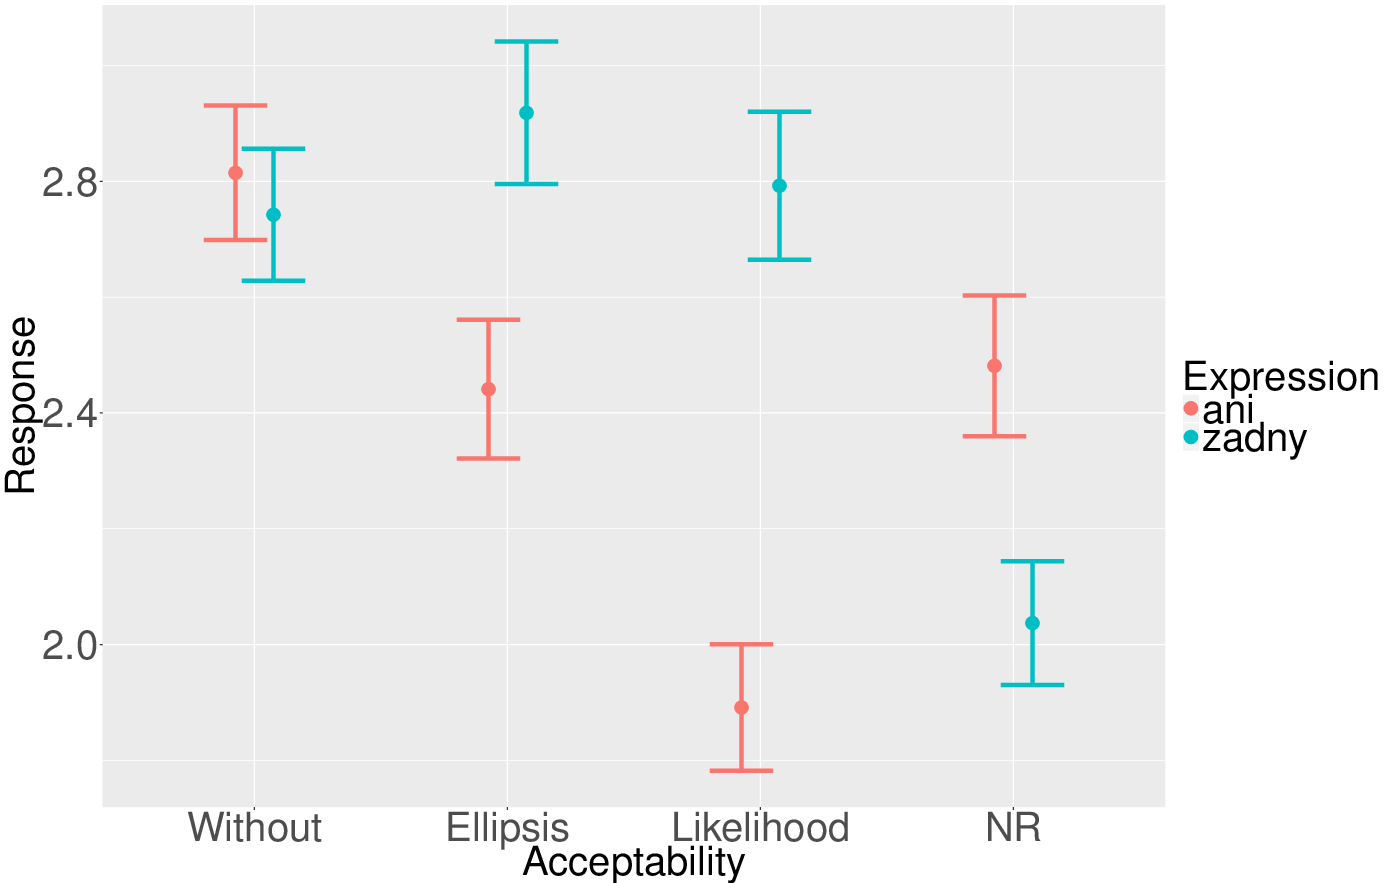
\includegraphics{include/mean-sum.png}
\caption{Experiment 3}
\end{figure}

The theoretical explanation of this known difference is usually explained via possible reconstruction of n-words and un-availability of reconstruction for NPIs. Because NPIs are usually not able to reconstruct under a possible licensor in their scope (deSwart 1998) like in the following example where NPI \textit{any} student in the cleft cannot reconstruct to its base object position under the quantifier \textit{no professor} which would license it. 

\ex.*It is any student that no professor like.

We further elaborated the fragment answer distinction in Experiment 3 (DETAILS: ) where we provided more contextual informations like in the example item \Next. But there the correlation disappeared: see the Figure XXX -- conditions FragNPI vs. FragNword with no difference in acceptability.

\ex. Koho vyhodil profesor Palný včera ze zkoušky?\\
whom fired prof Palný yesterday from exam? \a. Žádného studenta.\\
n-ADJ student \b. Ani jednoho studenta.\\
NPI one student

\begin{figure}
\centering
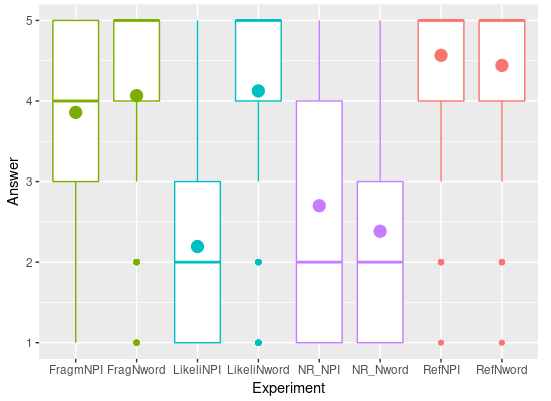
\includegraphics{include/Rplot04.png}
\caption{Experiment 4}
\end{figure}

The ability of n-words to appear as fragmentary answers is usually taken as the standard distinction against NPIs. But in a recent paper  \cite{fualuaus2016fragment} observes a strikingly related phenomen: she claims (based on data from many strict neg-concord languages) that in strict neg-concord languages n-word answers to negative questions can have (surprisingly) Double Negation (DN) reading. This observation goes again the the n-words vs.~NPIs criterion as it falsifies the second part of it. I checked FALAUS's claims with 10 native speakers of Czech and they are valid -- see an example \Next: there seems to be even a preference (8/10) for the DN reading -- \Next[a] but the negative concord reading \Next[b] is considered possible for 2 out of 10 speakers. 

\ex. Kdo nepřečetl žádný článek? Nikdo.\\
who neg.read n-ADJ article n-person \a. NC (2/10):
\(\neg \exists xy[Person'(x) \wedge Article'(y) \wedge Read'(x,y)] \equiv \forall x[Person'(x) \rightarrow \neg \exists y[Article'(y) \wedge Read'(x,y)]]\)
\b. DN (8/10):
\(\neg \exists x[Person'(x) \wedge  Article'(y) \wedge \neg Read'(x,y)] \equiv\forall x[Person'(x) \rightarrow \exists y[Article'(y) \wedge Read'(x,y)]]\)

FALAUS solve the availability of DN reading via postulating another (focus-related) position for covert negation (CN): in the left periphery of a clause as in the tree in \Next. The position is according to FALAUS licensed via n-word movement to the left peripheral position above TP. A negation in the left periphery is a second negation in a sentence, next to the reconstructed negation from the question. So the first negation in \Last[b] is the interpretation of covert negation, the second one of the verbal negation. If we follow FALAUS, we can explain the puzzling disappearance of contrast between n-words and NPI (Experiment 3) as a consequence of the covert negation -- if such a negation appears in a clause, the NPIs are licensed because they don't need to reconstruct under the scope of verbal negation and then the contrast between n-words and NPIs disappears.


\ex.
\(\Tree[[.CN ] [[.FOC n-word ][.TP [] [.NegP [. SN ] [.VP [.V ] n-word ]]]]]\)

There are many questions raised by postulating such covert negation, especially w.r.t. possible over-generation -- at the end n-words in strict negative concord languages cannot appear in sentences without negation but postulating covert negation leaves this robust observation unexplained. FALAUS tries to resolve such problems by restricting the covert negation only to strict set of cases, all somehow related to focus movement of n-words to the left periphery. I tried to verify her claims and conducted a small survey again with 10 speakers of Czech and it seems that FALAUS general idea is confirmed with an interesting twist. Let's start with a basic case -- \Next is interpreted only with NC reading as is visible from the ranking in \Next[a] and \Next[b] -- double negation is simply non-existent. 

\ex. Nikdo ničemu nevěří.\\
n-person n-thing neg.believes \a. NC:
\(\forall x[Person'(x) \rightarrow \neg \exists[Entity'(y) \wedge Believes'(x,y)]]\)
\b. *DN:
\(\forall x[Person'(x) \rightarrow \exists[Entity'(y) \wedge Believes'(x,y)]]\)

But in case of information structure manipulation like in \Next, which is even affirmative sentence, the double negation reading surprisingly emerges. The similar pattern is observed in \NNext. The sentences moreover seems to have the double negation reading only. This confirms FALAUS's hypothesis about focus position of the CN: \Last where there is no object movement to the left periphery (unlike in \Next and \NNext) has only the expected NC. It is not possible to explore more details of this interesting appearance of double negation reading in a negative concord language like Czech but more importantly: it seems to be reasonable to postulate another position for negation in the left periphery of a clause, such a position (because it is somehow licensed via focus) can the blur the picture of fragmentary answer criterion.

\ex. V nic nikdo nevěří.\\
in n-thing n-person believes \a. NC (0/10):
\(\forall x[Person'(x) \rightarrow \neg \exists[Entity'(y) \wedge Believes'(x,y)]]\)
\b. DN (10/10):
\(\forall x[Person'(x) \rightarrow \exists[Entity'(y) \wedge Believes'(x,y)]]\)


\ex. Nic při té zkoušce nikdo nenapsal.\\
n-thing at the exam n-person neg.wrote \a. NC (0/10):
\(\forall [... \neg \exists ...]\) \b. DN (10/10):
\(\forall [... \exists ...]\)

Summary of this section: there seems to be some evidence for classifying \textit{ani} as NPI and \textit{žádný} as n-word which stems from the fragment answer experiments. When the results diverge from expected dichotomy, there seems to be a reasonable explanation via postulation of a second covert negation in a sentence.

\hypertarget{likelihood-scenarios}{%
\subsection{Likelihood scenarios}\label{likelihood-scenarios}}

The last environment discussed in this article concerns the semantic properties of sentences where n-words vs. NPIs occur. The straightforward predictions are the following:

\begin{enumerate}
  \def\labelenumi{\arabic{enumi})}
  \tightlist
  \item
    n-words (licensed in syntax) shouldn't be sensitive to logical properties of
    their environment (they require just sentential/verbal negation)
  \item
    NPIs are licensed in semantics by definition are dependent on semantic properties like DE, anti-additivity, etc.
\end{enumerate}

I will pursue the line of treating apart NPIs from n-words via the NPI sensitivity to monotonicity and likelihood. And I will base my reasoning on a very influential theory of NPI licensing NPI licensing, so called \textbf{simple
  \emph{even} hypothesis of NPI licensing} (\citealt{heim1984note},  \citealt{krifka1995semantics}, \citealt{crnivc2014against}). The theory describes NPIs using the following three ingredients:

  \begin{itemize}
  \tightlist
  \item
    NPIs associate with covert \emph{even} -- the formalization can be via a formal [$even$] feature carried by the NPIs, etc.
  \item
    NPIs (like focused element) generate sets of possible alternatives
  \item
    covert \emph{even} associates with the alternatives and generates
    presupposition of its prejacent being the least probable member of
    the set of alternatives (entailing all the alternatives) -- in case of association with \textit{even}
  \end{itemize}

The immediate predictions of Heim/Crnič theory is that NPIs should be sensitive to probability and entailing properties (where the first and the second one are logically related: a proposition \textit{p} cannot be more likely than a proposition \textit{q}, if \textit{p} entails \textit{q}: intuitive illustration -- \textit{p} being \textit{Rambo killed 100 enemies}, \textit{q} being \textit{Rambo killed 99 enemies}, \textit{p} entails \textit{q} and \textit{p} is less likely than \textit{q}; \textit{q} doesn't entail \textit{p} and is more likely than \textit{q} -- see CRNIC for details of relating entailing and likelihood). The theoretical intricacies away, the prediction that NPIs should be sensitive to logical properties like entailing or probability while n-word not is uncontroversial, see the following table for next visualization of this prediction.

\begin{longtable}[]{@{}ll@{}}
\toprule
property/item & entailment/probability\tabularnewline
\midrule
\endhead
n-words & *\tabularnewline
NPIs & \(\checkmark\)\tabularnewline
\bottomrule
\end{longtable}


And we tested exactly this prediction in Experiment 2 and Experiment 3. In both we found strong correlation of \emph{ani} and probability. As a side note: a corpus survey (the biggest national Czech corpus,  \href{https://korpus.cz/}{Czech national corpus}) confirms the likelihood sensitivity of \textit{ani} -- a prototypical example in \Next shows that \textit{ani} usually associates with weak scalar items (\textit{ani jeden} is the second most frequent collocation, the first another minimizer \textit{ani slovo} `not a single word'). which via scalar reasoning entails all other scalar alternatives ($\neg \exists X[Customer'(X) \wedge \#X=1 \wedge Enter'(X)] \rightarrow \neg \exists X[Customer'(X) \wedge \#X>1 \wedge Enter'(X)]$). And due to this entailment the sentence with \textit{ani} and weak element associated with \textit{ani} is the least probable (entailing all other alternatives).

\ex. tento nyní úspěšný podnikatel {[}\ldots{}{]} v prvním měsíci neměl
ani jednoho zákazníka\\
this now very succesfull businesman {[}\ldots{}{]} in first month didn't
have {[}NPI one customer{]}

In the Experiment 2 we tested acceptability of \emph{ani} with strong scalar items -- example item in \Next where the scale of catholic hierarchy is most probably $\langle priest, bishop, cardinal\rangle$ -- \textit{cardinal} being high scalar item in any case. The scale entails contextual (not proper formal logical) entailment due to the facts of world we know the following implicational hierarchy: $\exists x[BecomeCardinal'(x) \rightarrow BecomeBishop'(x) \rightarrow BecomePriest'(x)]$ and its reversal $\exists x[BecomePriest'(x) \not\rightarrow BecomeBishop'(x) \not\rightarrow BecomeCardinal'(x)]$. To acquire the grade of cardinal entails acquiring (ceteris paribus) acquiring all lower ranks of catholic hierarchy but not the other way round. The scalar item \textit{cardinal} is the strongest (in the ad hoc scale), it entails all other items in the scale and is consequently least likely (which fits the natural intuitions). If \textit{ani} prefers weak/least-likely scalar items, it should be degraded with strong items, while n-words (as they are not picky about semantic environments) should be more acceptable.

\ex. (\ldots{}) nestal se \textbf{ani/žádným} kardinálem\\
`He didn't become even a cardinal.'

And we found out that people strongly preferred \emph{žádný} (n-word) with strong scalar items. The reason is that n-words do not have semantic requirements unlike NPIs: \textit{ani} prefers weak scalar items. The statistic results of Experiment 3 are in the FIGURE, the pertinent condition \textsc{likelihood}: \textit{ani} (red) had mean acceptability very much below n-word's mean acceptability (blue) around 2.8. 

\begin{figure}
\centering
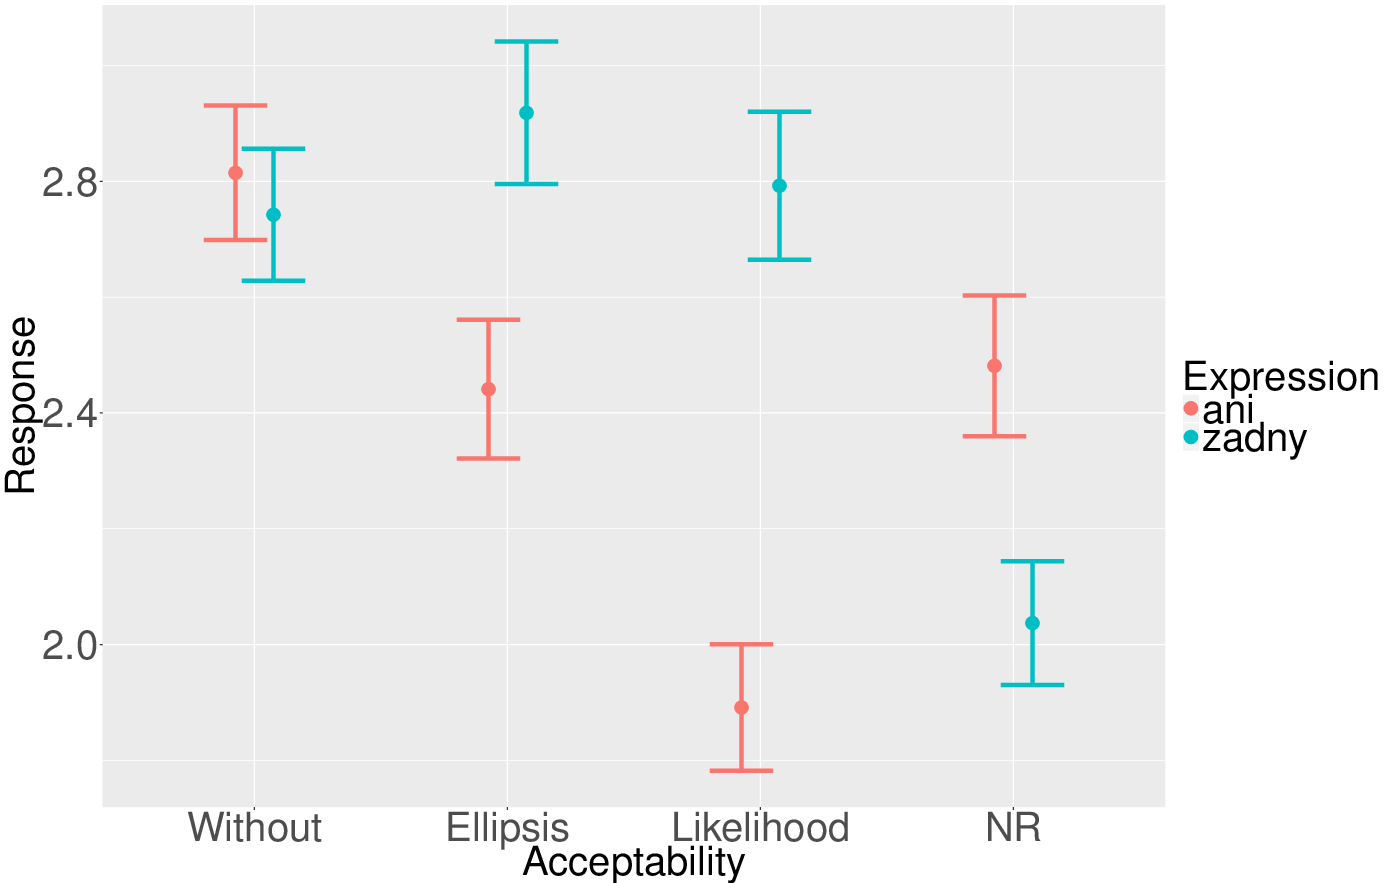
\includegraphics{include/mean-sum.png}
\caption{Experiment 3}
\end{figure}

Experiment 3 was partially an ellaboration of Experiment 2 -- while Experiment 2 used acceptability task, in Experiment 3 we used the truth value judgment task in case of testing likelihood properties of \textit{ani}. An example item is in \Next. Again we tested how much worse is acceptability of strong scalar items with \textit{ani}. In this scenario the scale is $\langle PhD,MA,BA\rangle$: here the scale is contextually based on the likelihood of passing the exam (if the scale would be based simply on academic hierarchy, as in the acceptability testing in \Last, it would be $\langle BA,MA,PhD\rangle$ but in \Next the scale is reversed as passing the exam is prototypically negatively correlated with the academic rank). The scale is (due to the context) again based on contextual entailment: $\forall x[BA'(x) \rightarrow  Pass'(x)] \rightarrow [\forall x[MA'(x) \rightarrow Pass'(x)] \rightarrow \forall x[PhD'(x) \rightarrow Pass'(x)]]$. Therefore \textit{ani} associates again with the strongest scalar item (in positive version of a tested sentence entailing all its scalar alternatives), therefore being the least likely. And as the statistical summary in FIGURE shows (the relevant condition \textsc{Likeli\_NPI} s. \textsc{Likeli\_Nword} -- blue color), speakers again preferred n-words to \textit{ani} NPIs.  This again follows from the \textit{ani} semantic requirements (being least likely among alternative scalar items)  vs. n-words which don't have any semantic sensitivity and are therefore more acceptable than \textit{ani}. 

\ex. Scenario: prof. Novák yesterday examined an easy course which B.A.,
M.A.~and Ph.D.~students attend. Ph.D.~students pass the exam always,
M.A.~in most cases but B.A. only seldomly. \a. Včerejší zkoušku u prof.
Nováka nesložili \textbf{ani/žádní} bakaláři.\\
yesterday exam at prof. Novák neg.passed NPI/n-Adj B.A.-students

\begin{figure}
\centering
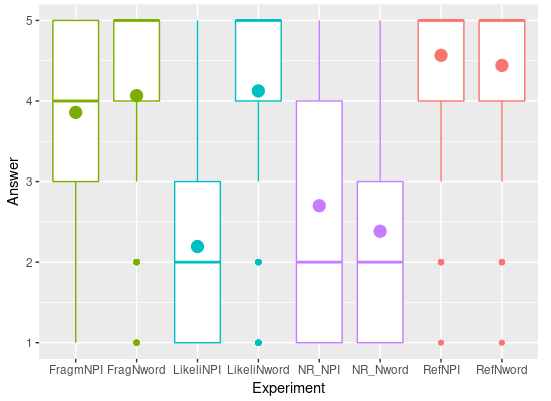
\includegraphics{include/Rplot04.png}
\caption{Experiment 4}
\end{figure}

Empirically the both experiments strongly support the classification of \textit{ani} as an NPI which associates with weak scalar items and \textit{žádný} as n-word licensed in syntax (and consequently without any particular semantic sensitivity).

\begin{longtable}[]{@{}ll@{}}
\toprule
property/item & probability\tabularnewline
\midrule
\endhead
\emph{žádný} & *\tabularnewline
\emph{ani} & \(\checkmark\)\tabularnewline
\bottomrule
\end{longtable}

The theoretical explanation of \textit{ani} being the NPI which obligatorily selects weak scalar items can be the following. First thing to note is that the facts observed in the experiments are only a piece of a bigger pattern where \textit{ani} competes in some environments with another scalar particle \textit{i} `even'. In a recent Experiment (\citealt{docekalsafratovaoli}) we experimentally confirmed that \textit{i} obligatorily selects strong scalar items, while \textit{ani} weak items. Illustrated on a data pattern close to the catholic hierarchy from Experiment 2 Czech native speakers are prone to the following judgments (where * should be understood as total un-acceptability in experiments, ?? as in-between-acceptability and $\checkmark$ as nearly total acceptability -- statistic noise away -- but of course only in case the judgments are related to the set up scale, catholic hierarchy in \Next).

\ex. \a. upward entailing contexts:
\a. Petr se nakonec stal $\checkmark$i kardinálem/??i knězem.
\b. Petr se nakonec stal *ani kardinálem/*ani knězem.
\z.
\b. downward entailing, non anti-additive contexts:
\a. Jestli se Petr stal $\checkmark$i kardinálem/??i knězem, tak \ldots
\b. Jestli se Petr stal *ani kardinálem, tak \ldots
\z.
\c. downward entailing, anti-additive contexts:
\a. Petr se nakonec nestal *i kardinálem/*i knězem. 
\b. Petr se nakonec nestal ??ani kardinálem/$\checkmark$ani knězem.

The pattern we observe is the following: \textit{i} in upward entailing contexts and downward entailing contexts prefers strong elements on scale but it is un-acceptable with weak or strong scalar items in anti-additive contexts; \textit{ani} prefers weak scalar items in anti-additive contexts but it is un-acceptable in upward entailing contexts with both weak and strong scalar items. Such pattern is explainable (following the logic of argumentation in CRNIC) as \textit{i} and \textit{ani} spelling out the following features:

\ex. \a.\textit{i} \ldots [\textsc{even}]
\b. \textit{ani} \ldots [\textsc{even},\textsc{aa}]

The feature [\textsc{even}] requires the association with covert \textit{even} defined below. The feature [\textsc{aa}] requires the item to occur in the anti-additive environment. The items form a scale in \Next and compete for insertion via the usual Maximize presupposition principle in \NNext.

\ex. $\langle i,ani\rangle$

\ex. MAXIMIZE PRESUPPOSITION

\ex. \(\llbracket even\rrbracket ^w (C)(p)\) is defined only if
\(\forall q \in C[q \neq p \rightarrow q >_{likely} p]\)

The observed distribution of \textit{i}/\textit{ani} and their strong/weak association is explainable as follows:

\begin{enumerate}
	\item upward entailing environments: \textit{i} is licit but only with strong scalar items as then the \textit{even} presupposition is satisfied, \textit{ani} cannot be inserted as UE environments clash with \textit{ani} [\textsc{aa}] feature;
	\item downward entailing environments: \textit{i} is licit with the \textit{even} scoping below DE operator:  {[} \(\rightarrow\) {[}{[}even C{]} antecedent \ldots{} \textit{i} \ldots ] consequent ], \textit{ani} cannot be used due to the [\textsc{aa}] feature requirement;
	\item anti-additive environments: \textit{i} cannot be inserted because Maximize Presupposition dictates the insertion of the most specific item (\textit{ani} in this case), \textit{ani} associates with weak scalar items: the scope [even C] [$\neg$ \ldots \textit{ani} \ldots]
	\item the association of \textit{i}/\textit{ani} with 'wrong' scalar items is perceived as bad (??) but not totally ungrammatical -- weak scalar item for \textit{i} in upward entailing contexts and strong scalar items for \textit{ani} in anti-additive environments;
	
\end{enumerate}

The last point seems to point at the existence of possible reversed scoping: [even C][$\rightarrow$ [antecedent \ldots \textit{i} \ldots] consequent ] for \textit{i} and  [$\neg$ [even C] \ldots \textit{ani} \ldots] for \textit{ani} which would explain their allowed (even if not preferred) 'crossed' association. But as it was confirmed by Experiment 2 and Experiment 3 \textit{ani} associates with weak items, while \textit{i} with strong scalar items (see DOCEKAL \& SAFRATOVA for details) by default. This default scope exchange of \textit{i}/\textit{ani} which happens exactly in anti-additive contexts (\textit{i} prefers strong elements, \textit{ani} weak element but only in scope of negation -- negation being the anti-additive licensor in 99\%) reveals their unified semantics where the flip-flop is a consequence of entailment/likelihood reversal caused by the negation. The only difference between \textit{i} and \textit{ani} is the formal feature [\textsc{aa}] which formalizes the morphological incorporation of negation into \textit{ani}.  It would be possible to encode the scope differences via different features ([\textsc{solo}] of CRNIC for the weak elements) but such a move would miss the nice competition pattern which emerged from the data: namely \textit{i} is in principle expected in anti-additive environments but cannot be inserted as a consequence of \textit{ani} being more specific ([\textsc{even,aa}]).

\hypertarget{summary}{%
\subsection{Summary}\label{summary}}

Let's end this article by answering the question asked at the beginning: do  n-words and strong NPIs co-exist in natural language. And if yes (in some languages like English they do exist for sure), does this distinction hold even in strict neg-concord languages where the boundary between strong NPIs and n-words is even more subtle? The experiments, their results and their theoretical interpretation described in this article brings very strong support of the existence of both classes of negatively dependent expressions even in strict neg-concord languages like Czech. This result allows us to maintain the standard assumptions concerning n-words (they are licensed syntactically) and   NPIs (they are licensed in semantics/pragmatics). More importantly, the data patterns of Czech NPIs seem to strongly favorize the NPI theories which base their licensing on concepts like  anti-additivity and likelihood (\citealt{zwarts1998three} in the first case, \citealt{heim1984note} and \citealt{crnivc2014against} in the second). Another issue touched in this article is un-reliability of our intuitions: it seems that distinguishing between n-words and strong NPIs has to be based on such subtle date which can dealt only by experimental methods. The subtlety of judgments can explain differing stances on this distinction in the previous literature where such opposing views as: n-words are a subclass of NPIs (\citealt{ladusaw1992expressing}, \citealt{fualuaus2016fragment} a.o.) versus n-words are a separate class (\citealt{zeijlstra2008negative} and \citealt{giannakidou2017landscape} a.o.) were maintained. There's another pertinent question raised by the data: do all speakers agree with respect to the distinction between n-words and strong NPIs? And if no, is there a real dialectal variation or at least some correlation? The results of our experiments in fact bear direct evidence on this fascinating question  but the space of this article is alas filled completely.

\bibliography{bibliography}
\bibliographystyle{chicago}


\end{document}
